\documentclass[10pt,a4paper,twoside]{article}
% IMPORTS AND LIBRARIES
\usepackage[utf8]{inputenc}
\usepackage[english]{babel}
\usepackage{amsmath}
\usepackage{amsfonts}
\usepackage{amssymb}
\usepackage{graphicx}
\usepackage{hyperref}
\usepackage{booktabs}
\usepackage[math]{blindtext} % generates text for document filling purposes
\usepackage{lipsum}
\usepackage[left=4cm,right=4cm,top=2cm,bottom=2cm]{geometry}
% DOCUMENT SETUP
\author{Ludovic Charleux}
\title{\textsc{My first document}}
\date{Feb. 15th 2024}
% DOCUMENT
\begin{document}
\maketitle

\tableofcontents

\section{Introduction to \LaTeX}
This is our first document.
We are so proud of it.
It deals about \LaTeX and writing stuff with it.
I need to write some more text here to show you some new ideas.
Again, I write useless stuff to populate our document.
I'm so happy !

\subsection{Sectionning documents is fun}
This is a new paragraph.
I have new stuff to say !

\subsection{Oh yes}
Again, I'm writing text.
\textbf{I like bold fonts.} % \textbf is for bold fonts.
\textit{And italics as well !} % \textit is for italics fonts

\section{Useful environments}

\subsection{Buletted lists and enumerations}

\begin{itemize}
  \item On thing.
  \item Another thing.
        \begin{enumerate}
          \item Ah yes, I can enumerate !
          \item And environments can be nested !
        \end{enumerate}
  \item Again, a bullet.
\end{itemize}

\section{Using maths in \LaTeX}

One basic way to write math in \LaTeX~ is to make standalone like this one:

$$
  f(x) = x^2
$$

\noindent And here, I can write text again.
Here is a more advanced example:

\begin{equation}
  u = \sum_{n=1}^{+\infty} v_n
  \label{eq:awesome_math}
\end{equation}

\noindent After the awesome Eq. \ref{eq:awesome_math}, it's possible to write equations inside the text because $\alpha = 5$ and this is because of the famous equation $x = \frac{2}{3}$.
As you can see, it is possible to put inline math.
Of course, there are advanced environments for things you will use in math like aligning equations:

\begin{align}
  A & = (a+b)^2        & + (a+b)(a-b)\nonumber \\
    & = a^2 + 2ab +b^2 & + a^2 - b^2
\end{align}

\noindent Underbraces are nice also:

\begin{equation}
  A = \underbrace{(a+b)^2}_{a^2 + 2ab +b^2}
  + \underbrace{(a+b)(a-b)}_{a^2 - b^2}
\end{equation}

\noindent And matrices as well:

\begin{align}
  \vec w & = \vec u \cdot \vec v         \\
         & =
  \begin{bmatrix}
    x_u & y_u & z_u
  \end{bmatrix}
  \cdot
  \begin{bmatrix}
    x_v \\ y_v \\ z_v
  \end{bmatrix}              \\
         & = x_u x_v + y_u y_v + z_u z_v
\end{align}


\section{Managing figures}

In \LaTeX, with the \textit{graphicx} package, we can include images like this 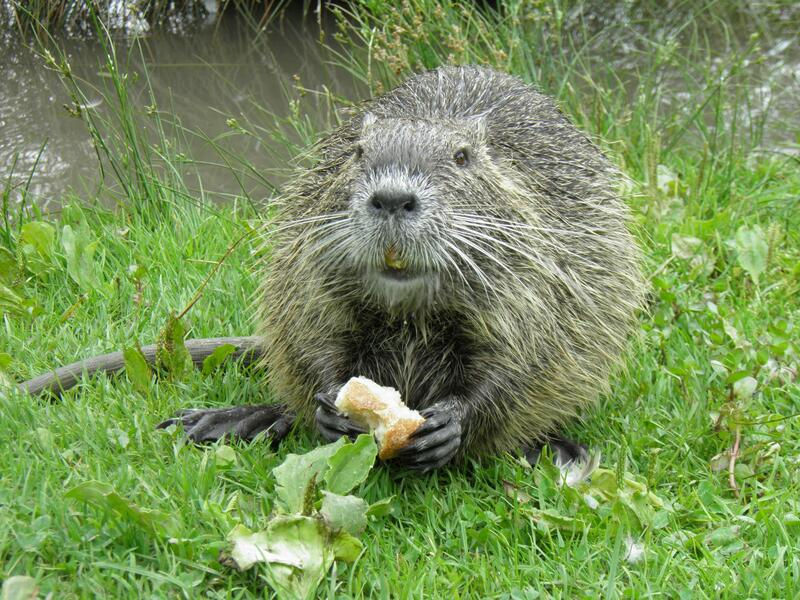
\includegraphics[width = 0.5cm]{figures/ragondin_small.jpg}.
In real life, you would like to have it as a standalone image like this one:

\begin{center}
  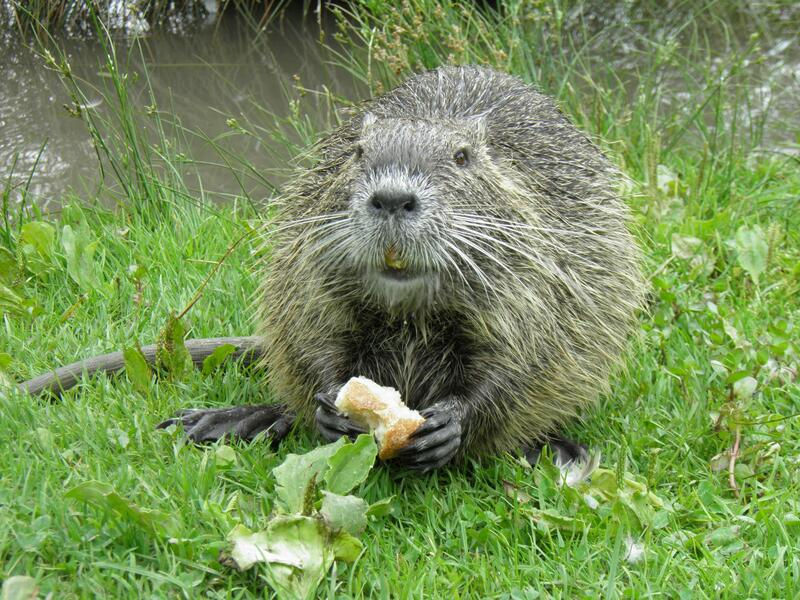
\includegraphics[width = .8\textwidth]{figures/ragondin_small.jpg}
\end{center}

\noindent An here we go again.
We can embed images in the text this way.
The Fig. \ref{fig:ragondin_explained} shows how to make a figure in \LaTeX .

\begin{figure}[hb]
  \begin{center}
    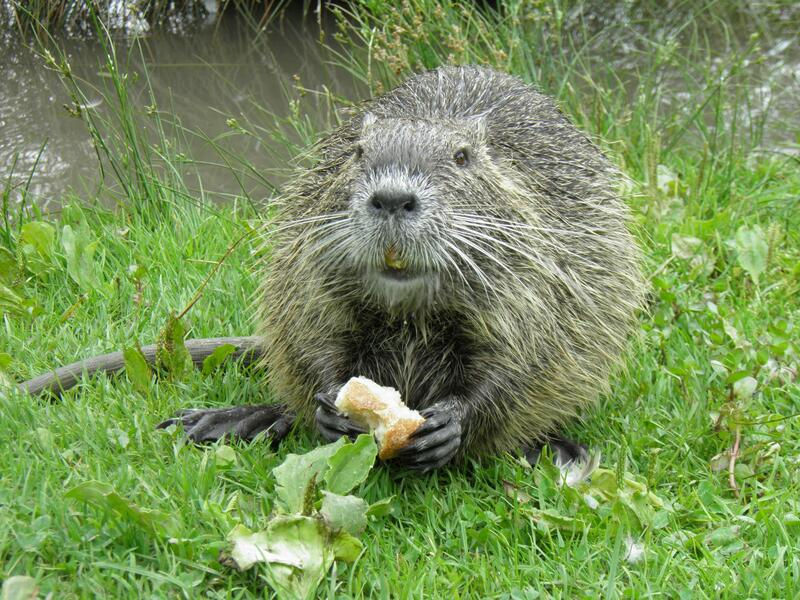
\includegraphics[width = .8\textwidth]{figures/ragondin_small.jpg}
    \caption{Here we have a figure with a caption in a floating environment.
      \blindtext[1]}
    \label{fig:ragondin_explained}
  \end{center}
\end{figure}


\blindtext[4]

\section{Tabulars and tables}

A table is simple, at least at the beginning.

\begin{center}
  \begin{tabular}{l|cr} % c = centerd, r = flush right, l = flush left
    \hline % Horizontal line
    Animal & Hase fur ? \\
    Rabbit & Yes        \\
    Turtle & No         \\
    \hline
  \end{tabular}
\end{center}

The same table with \url{https://www.tablesgenerator.com/}: % \includepackage{hyperref}

% Please add the following required packages to your document preamble:
% \usepackage{booktabs}
%\begin{table}[]
\begin{center}
  \begin{tabular}{@{}lcr@{}}
    \toprule
    \textbf{Animal} & \textbf{Has Fur ?} & \textbf{Will bite me ?} \\ \midrule
    Rabbit          & Yes                & No                      \\
    Turltle         & No                 & It depends              \\ \bottomrule
  \end{tabular}
\end{center}
%\end{table}


\section{Bibliography}

I can cite \cite{hawking1974black} documents like this.
Or this one also \cite{belczynski2012missing}.

% BIBLIOGRAPY
\bibliographystyle{plain}
\bibliography{my_bibliography.bib}


\end{document}